\documentclass[border=10pt]{standalone}
\usepackage{graphicx}
\usepackage{epstopdf}
\usepackage{mathptmx}
\usepackage{amsmath}

\begin{document}
\begin{minipage}{32cm}
\centering
\begin{minipage}[t]{0.49\linewidth}
\centering
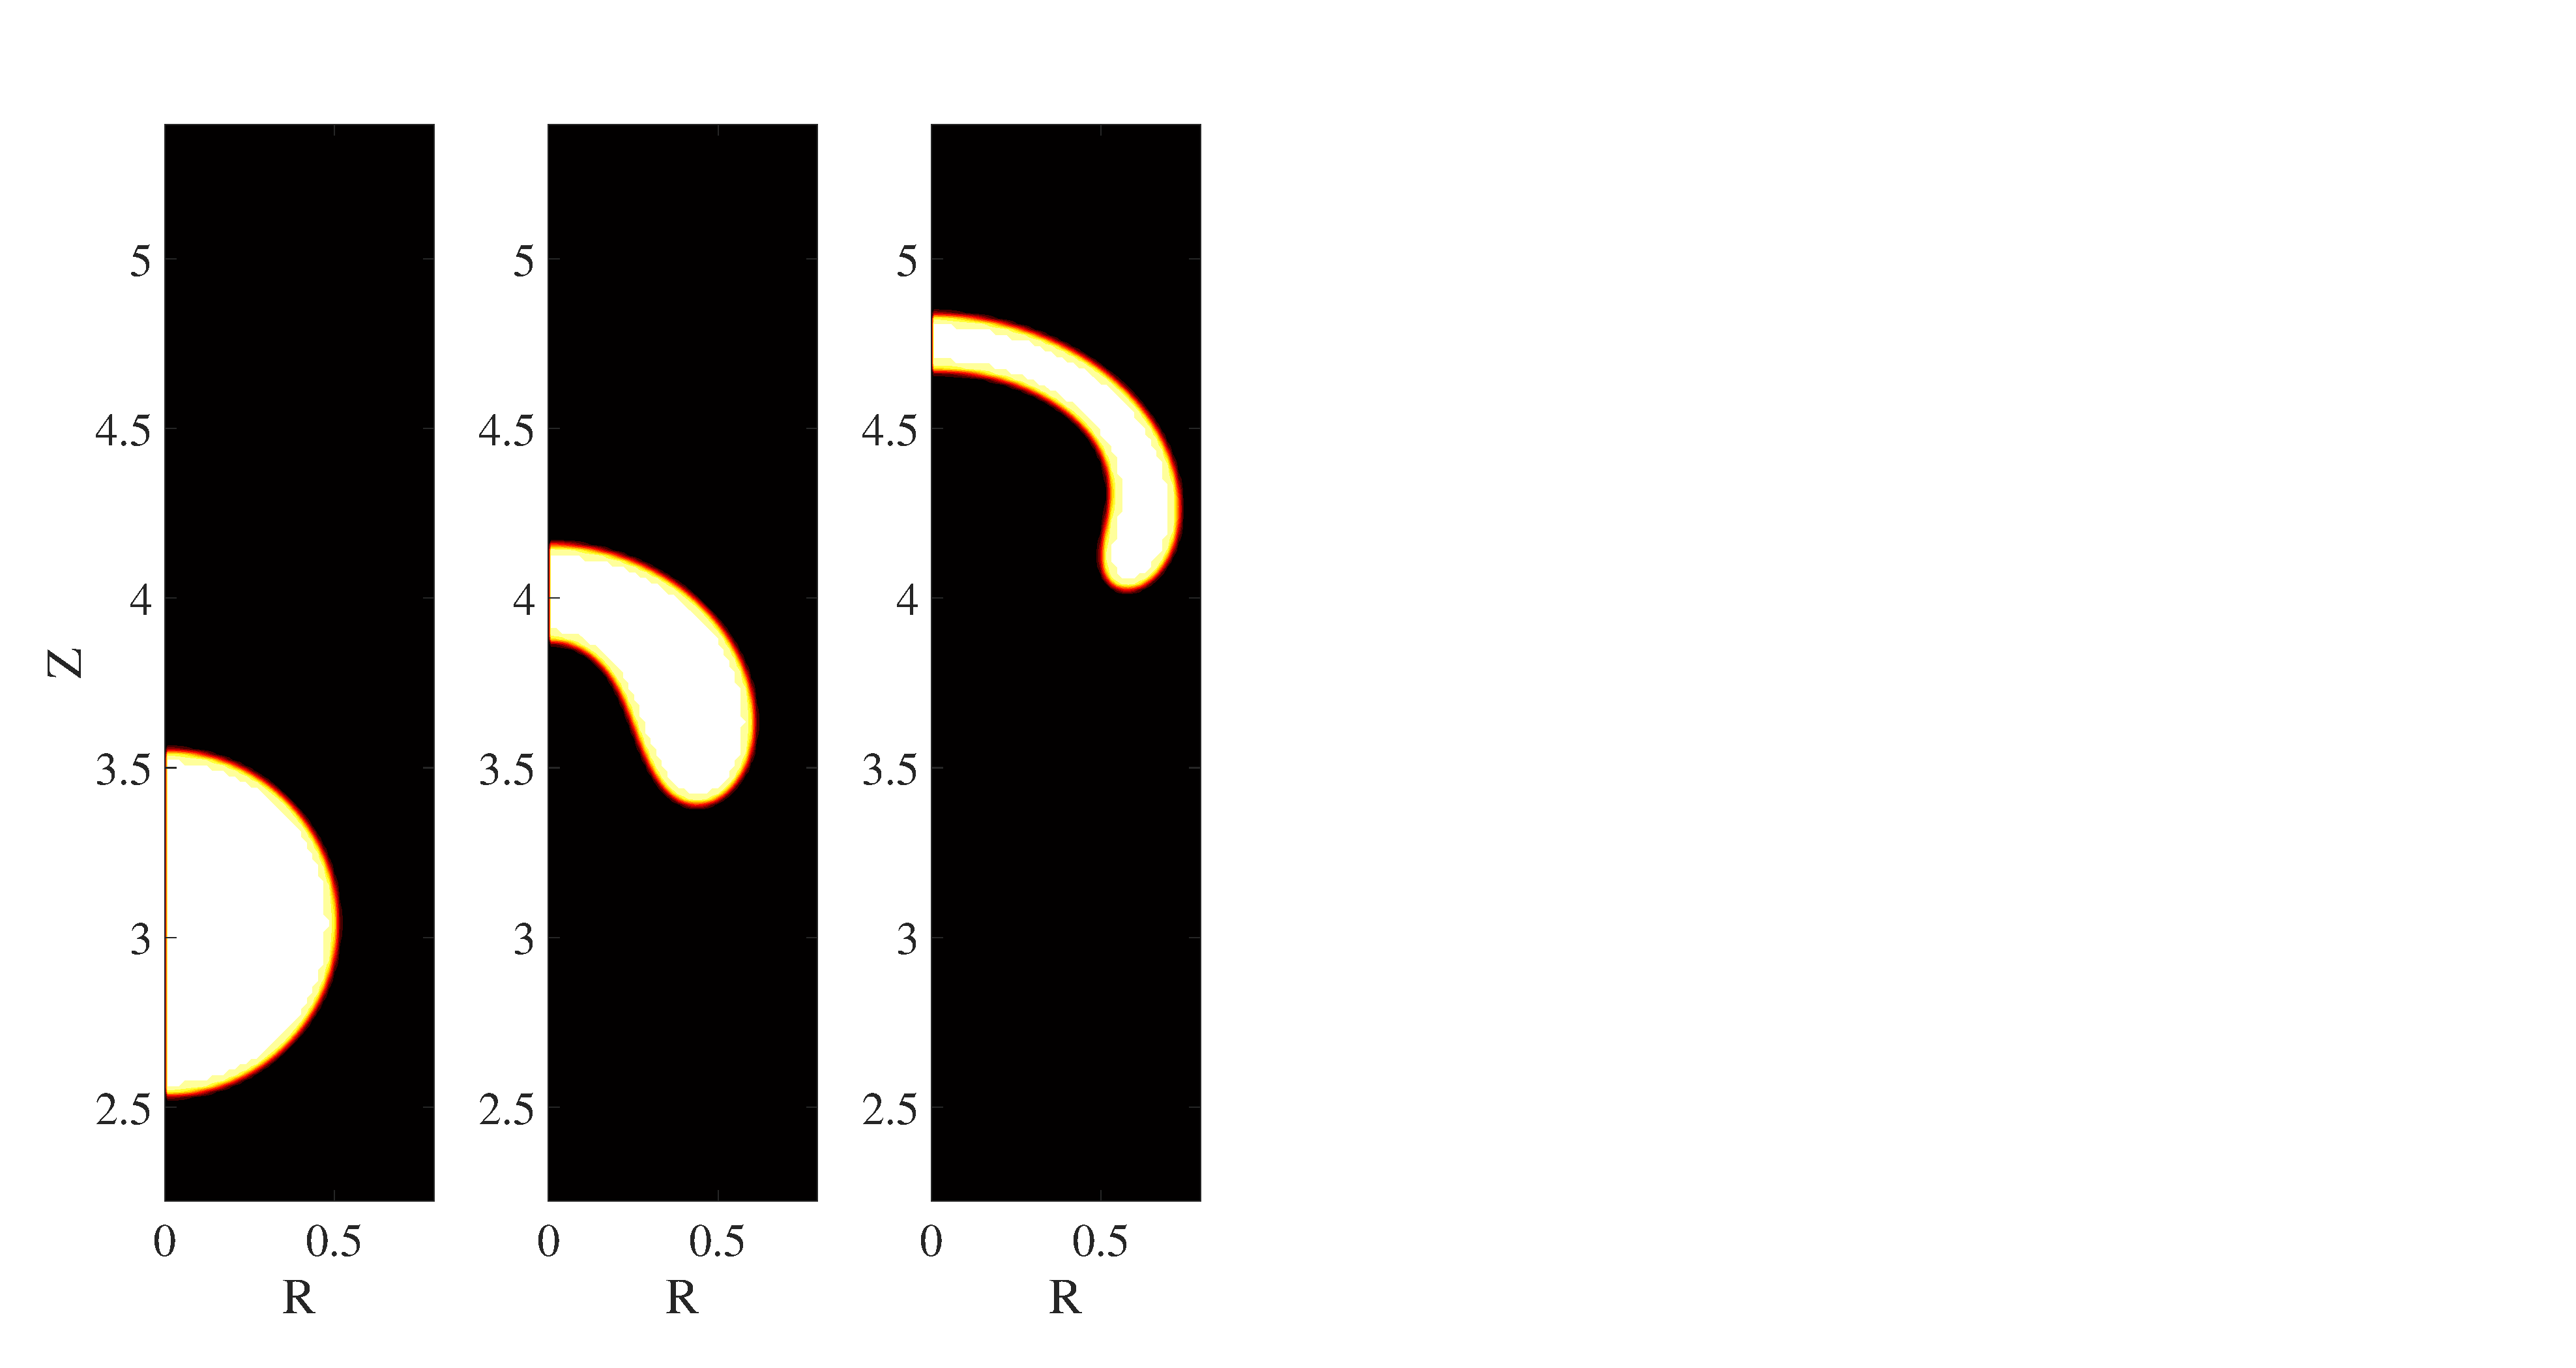
\includegraphics[scale=0.5,trim={0.8cm 1cm 0cm 1cm},clip]{Figure2a.eps}
\put(-920,450){\fontsize{20}{12}\selectfont\textbf{(a)}}
\end{minipage}
\hfill
\begin{minipage}[t]{0.49\linewidth}
\centering
\includegraphics[scale=0.5,trim={0.8cm 1cm 0cm 1cm},clip]{Figure2b.eps}
\put(-920,450){\fontsize{20}{12}\selectfont\textbf{(b)}}
\vspace{0.5cm}
\end{minipage}
\begin{minipage}[t]{0.49\linewidth}
\centering
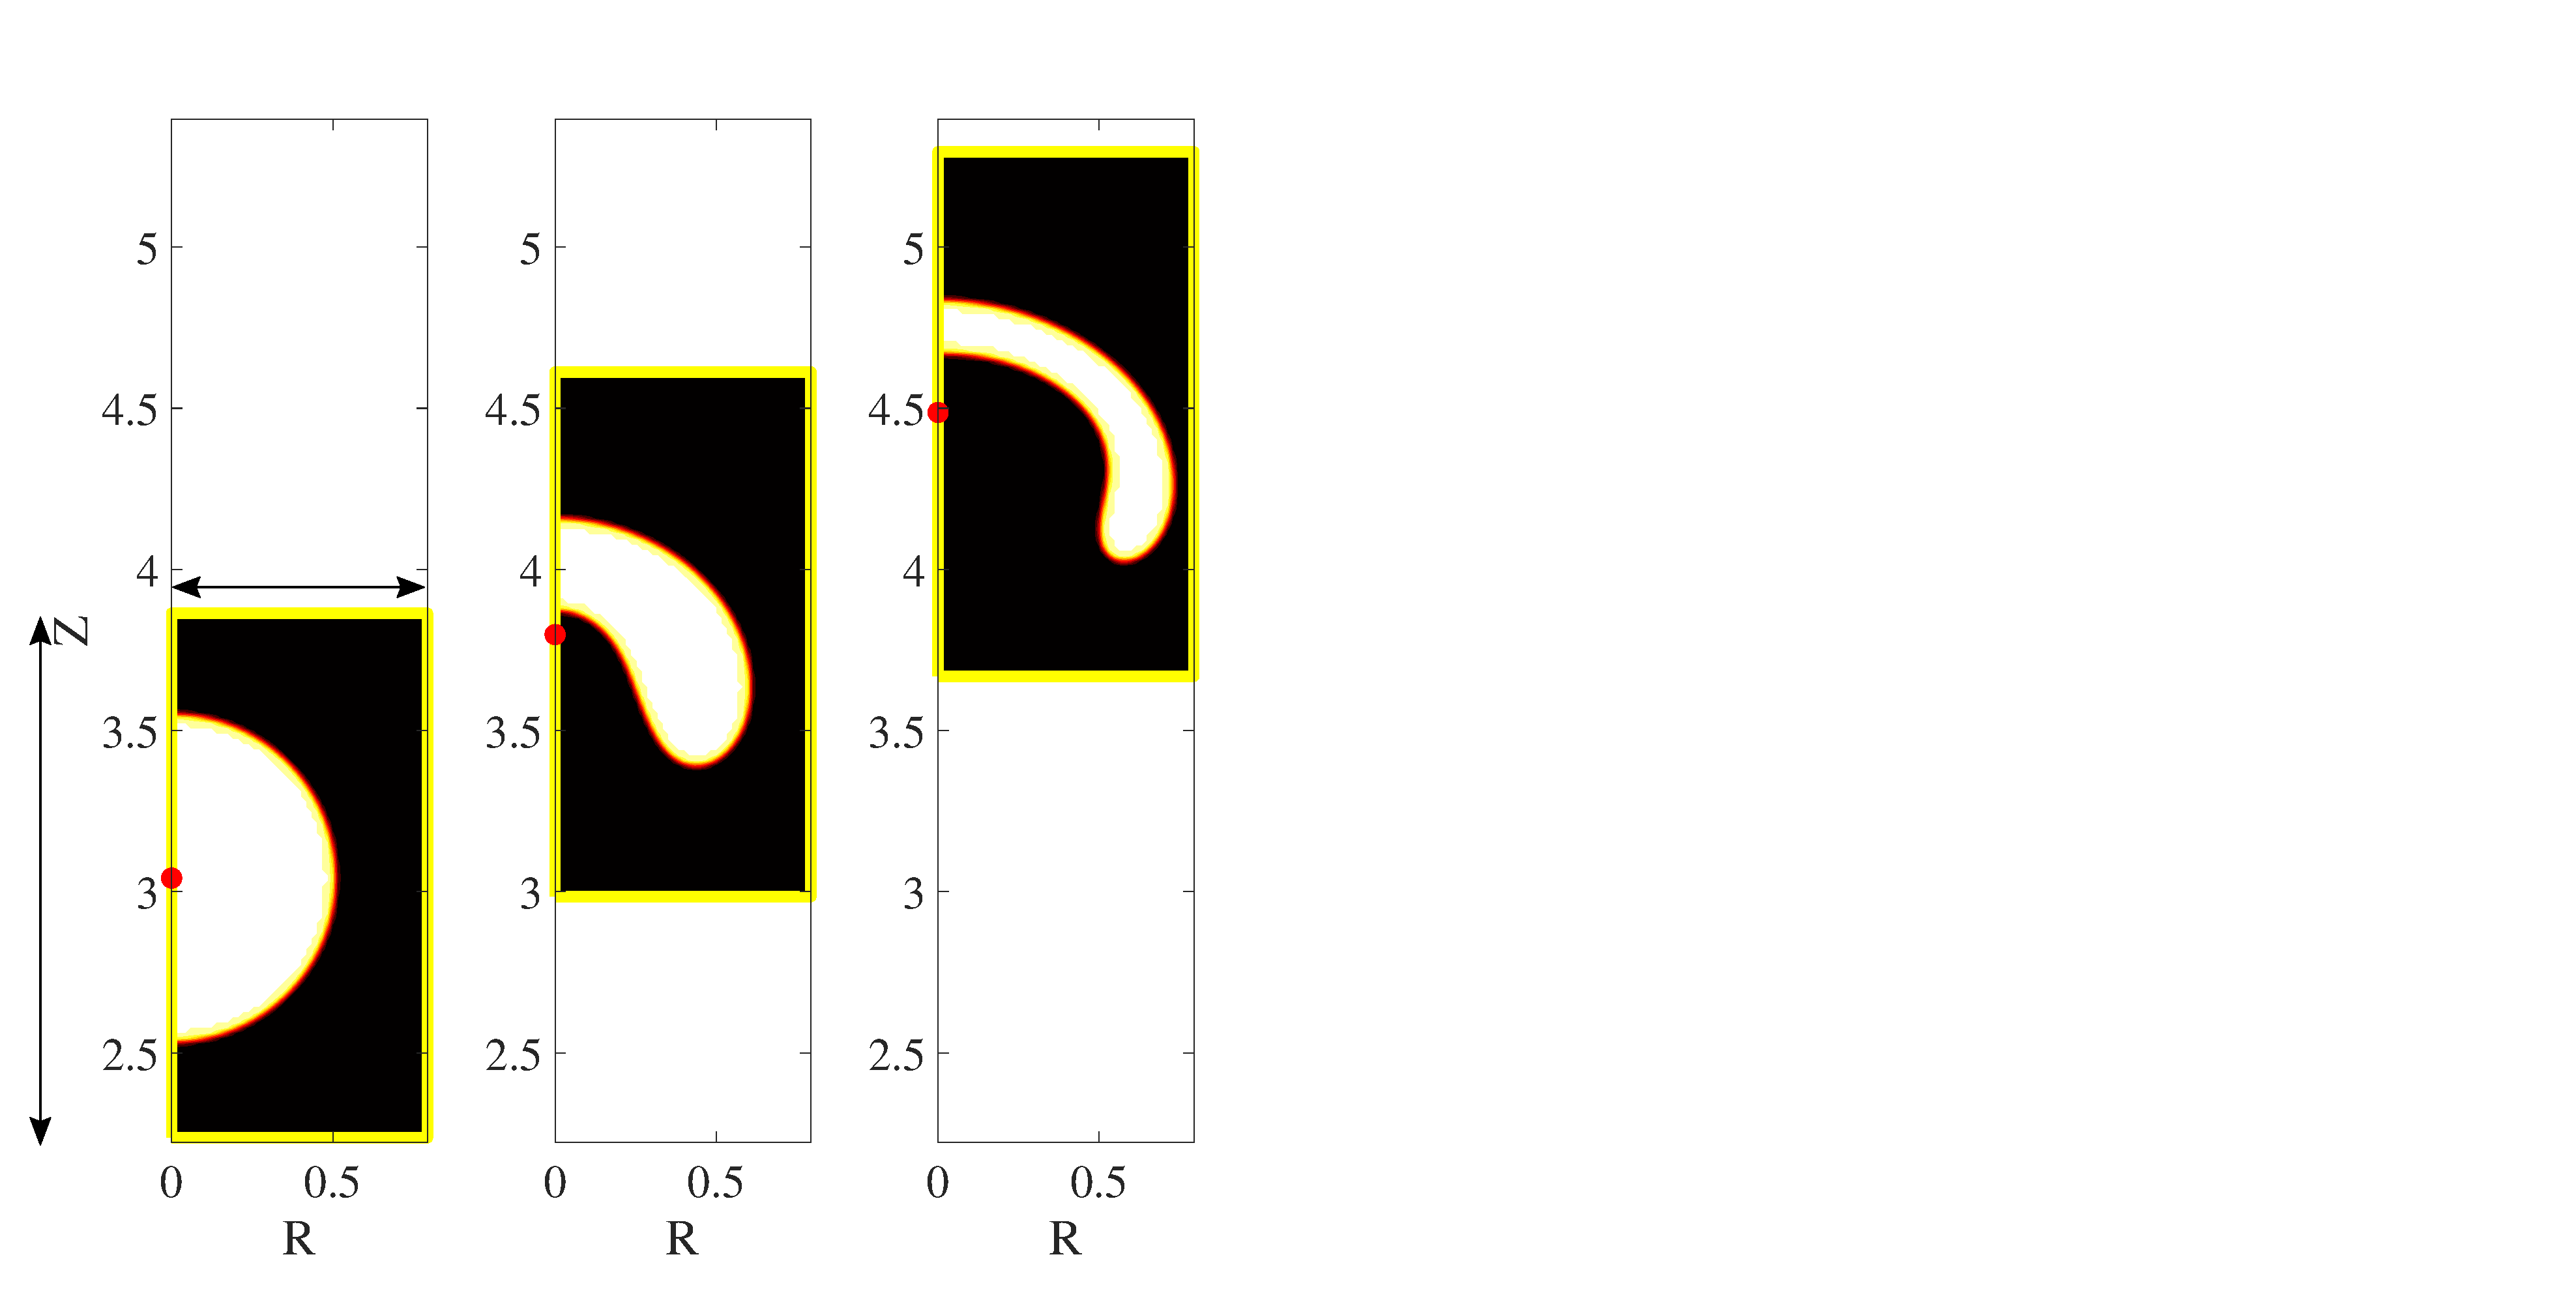
\includegraphics[scale=0.5,trim={0cm 1cm 0cm 1cm},clip]{Figure2c.eps}
\put(-920,430){\fontsize{20}{12}\selectfont\textbf{(c)}}
\put(-860,260){\fontsize{20}{12}\selectfont\textbf{0.75D}}
\put(-980,130){\fontsize{20}{12}\selectfont\textbf{1.5D}}
\end{minipage}
\end{minipage}
\end{document}
